\section{K-means Results}

\subsection{K-means Clusters}
\label{A_kmr_clusters}
\begin{lstlisting}[basicstyle=\footnotesize\ttfamily,numbers=none]
=== Run information ===

Scheme:weka.clusterers.SimpleKMeans -N 5 -A "weka.core.EuclideanDistance -R first-last" -I 500 -S 0
Relation:     KMeansReadyDataSet
Instances:    900
Attributes:   6
              unemploymentRate
              balanceOfPayments
              gdpPerInhabitant
              population
Ignored:
              year
              country
Test mode:evaluate on training data

=== Model and evaluation on training set ===

kMeans
======

Number of iterations: 47
Within cluster sum of squared errors: 26.785974154815772
Missing values globally replaced with mean/mode

Cluster centroids:
                                   Cluster#
Attribute           Full Data           0            1            2            3             4
                        (900)       (355)         (87)        (192)         (88)         (178)
=================================================================================================
unemploymentRate       8.4462      7.1908      16.3207       8.7537       4.4761        8.7321
balanceOfPayments    155.6269   -124.9762   -4056.8519   -1969.4913   14654.6009     -2101.605
gdpPerInhabitant   18079.6529  19416.3004   12195.1086      6943.75   43498.8636    17734.9806
population      17952543.9686 6887700.166 14437551.069 7818847.2542 5956189.9432 58599582.4831

Time taken to build model (full training data) : 0.1 seconds

=== Model and evaluation on training set ===

Clustered Instances

0      355 ( 39%)
1       87 ( 10%)
2      192 ( 21%)
3       88 ( 10%)
4      178 ( 20%)
\end{lstlisting}

\begin{figure}[h!]
  \centering
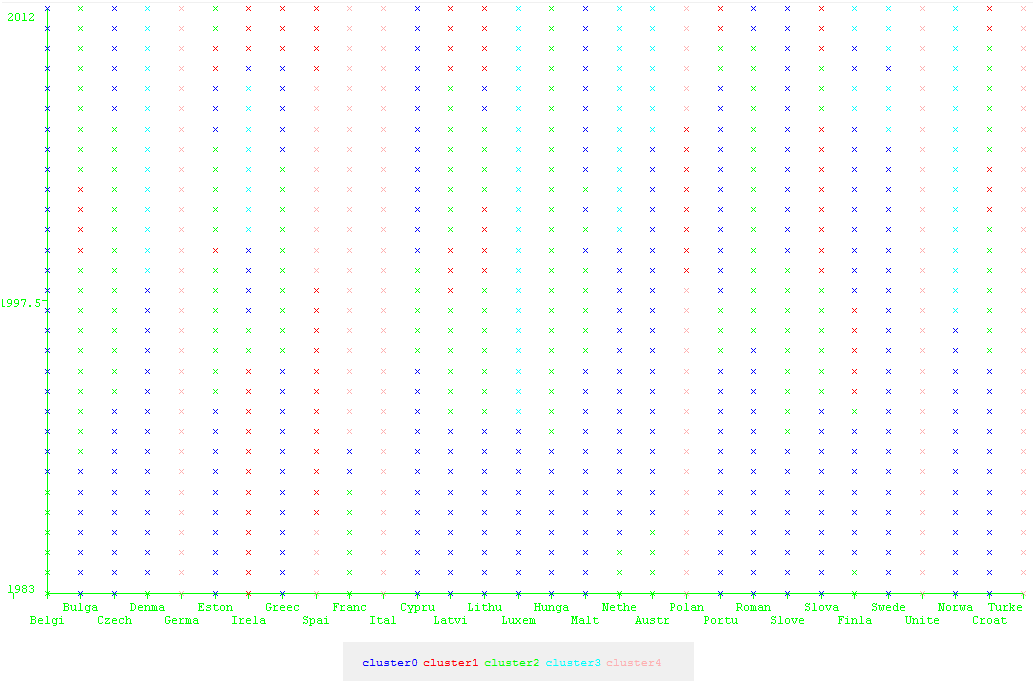
\includegraphics[angle=90,width=0.8\textwidth]{Appendix/Images/kMeans}
\caption{Graphical representation of what clusters the countries belong to at what year}
\label{fig:largeClusters}
\end{figure}

\subsection{K-means USA's Placement}
\label{A_kmr_usa}
\begin{lstlisting}[basicstyle=\footnotesize\ttfamily,numbers=none]
Cluster centroids:
                                   Cluster#
Attribute           Full Data           0            1            2            3             4
                        (900)       (355)         (87)        (192)         (88)         (178)
=================================================================================================
unemploymentRate       8.4462      7.1908      16.3207       8.7537       4.4761        8.7321
balanceOfPayments    155.6269   -124.9762   -4056.8519   -1969.4913   14654.6009     -2101.605
gdpPerInhabitant   18079.6529  19416.3004   12195.1086      6943.75   43498.8636    17734.9806
population      17952543.9686 6887700.166 14437551.069 7818847.2542 5956189.9432 58599582.4831

Time taken to build model (full training data) : 0.1 seconds

=== Model and evaluation on training set ===

Clustered Instances

4        1 ( 100%)

USA's data is:
2011,USA,8.9,-339793,34700,310544109,cluster4
\end{lstlisting}

\pagebreak